
\subsection{Waveguides}

\begin{figure}[h!]
    \centering
    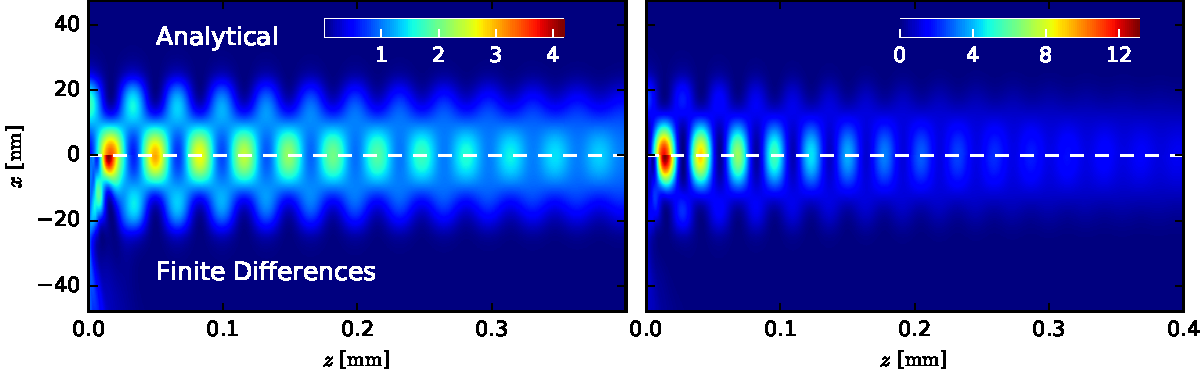
\includegraphics[width=1\textwidth]{analytical/analytical_waveguide}
    \caption{Comparison of intensity cross-sections of the analytical solutions far from the entrance with finite difference simulations of a symmetric slab waveguide (left) and a cylindrical waveguide (right). The waveguides consist of Germanium with vacuum cores of 48nm diameter. The initial condition is a plane wave with 12keV photon energy. Intensity values are plotted as relative to the intensity of the plane wave.}
    \label{fig:waveguide_fd_analytical_comparison}
\end{figure}


\subsubsection{Symmetric Slab Waveguide}

The slab waveguide is a waveguide consisting of a guiding layer with complex refractive index $n_1$ and thickness $d$ sandwiched between two semi-infinite cladding regions of complex refractive index $n_2$ where $\Re\, n_2 < \Re\, n_1$. We choose the orientation of the waveguide so the refractive index is a function of $x$ 

\begin{align*}
    n(x,z) = 
    \begin{cases}
    n_1 & \text{if } |x| \le d/2\\
    n_2 & \text{otherwise.}
    \end{cases}
\end{align*}

We find the analytical field inside the waveguide by first ignoring absorption and making the ansatz $\psi_{\vec x}(x,z) = \psi_m(x) \exp(i \beta_m z)$, where $\beta_m \in \mathbb{R}$ is called the propagation constant of mode $m$. Inserting this into the Helmholtz equation~\eqref{eq:helmholtz} gives us a one-dimensional differential equation for $\psi_{\vec x}(x)$

\begin{align*}
    \frac{\partial^2 \psi_m}{{\partial x}^2} = (\beta^2 - n^2 k^2) \; \psi_m.
\end{align*}

We demand the solutions to be symmetrical and to vanish as $x \rightarrow \infty$. A class of solutions satisfying these criteria is

\begin{align*}
    \psi_m = 
    \begin{cases}
    \cos(\kappa x) & \text{if } |x| \le d/2\\
    a \exp(\gamma (d/2 - |x|)) & \text{otherwise}
    \end{cases}
\end{align*}

where $\kappa = \sqrt{n_1^2 k^2 - \beta_m^2}$, $\gamma = \sqrt{\beta_m^2 - n_2^2 k^2}$ and $a = \cos(\kappa d/2)$ are positive real numbers. We call these solutions the symmetrical guided modes of the waveguide. Since the solutions must be contiguously differentiable we find the additional constraint 

\begin{align*}
\tan(\kappa d/2) = \frac{\gamma}{\kappa} = \frac{ \sqrt{k^2 (n_1^2 - n_2^2) - \kappa^2} }{ \kappa } \; , 
\end{align*}

which we call the characteristic equation of the waveguide. The propagation constants $\beta_m$ are determined by this equation. 

We now show that the characteristic equation has a finite number of $N$ solutions for $\kappa$. The left side is strictly monotonously increasing almost everywhere and jumps from $\infty$ to $-\infty$ with period in $2 \pi / d$ while the right side is strictly monotonously decreasing. Therefore there is exactly one intersection in every period of the left argument. Since $\gamma$ is real, $\kappa$ has the upper bound $k \sqrt{ (n_1^2 - n_2^2)}$, which also bounds $N$

\begin{align*}
   \left\lfloor \frac{ d \, k \sqrt{ (n_1^2 - n_2^2) } }{ 2 \pi } \right\rfloor \le N \le \left\lceil \frac{ d \, k \sqrt{ (n_1^2 - n_2^2) } }{ 2 \pi } \right\rceil.
\end{align*}

We can now reintroduce absorption by introducing an effective linear attenuation coefficient $\mu_m$~\cite{DissertationFuhse}

\begin{align*}
    \mu_m = \frac{1}{\lVert \psi_m \rVert_2^2} \int_\mathbb{R} \mu(x) \left| \psi_m(x) \right|^2 \text{d}x,
\end{align*}

where $\lVert \psi_m \rVert_2$ is the $L^2$ norm of $\psi_m$. Far away from the entrance the field in the waveguide consists only of the guided modes

\begin{align*}
    \psi(x,z) = \sum_{m=1}^{N} c_m \psi_m(x) \exp( i \beta_m - \mu_m z),
\end{align*}

where coefficients $c_m$ are determined by projecting the incident plane wave onto the guided modes

\begin{align*}
    c_m = \frac{1}{\lVert \psi_m \rVert_2^2} \; \int_\mathbb{R} \psi_m(x) \cdot \psi_0 \; \text{d}x,
\end{align*}

where $\psi_0$ is the field strength of the plane wave. In \figref{fig:waveguide_fd_analytical_comparison} (left) we see a comparison of the intensity of the analytical solution with a finite difference simulation for a waveguide consisting of Germanium with a Vacuum guiding layer at $E = 12\text{keV}$. We see that after a transient state the intensity profiles are almost identical. For a more detailed comparison and also for results acquired with the multi-slice Fresnel propagator see \lstinline{waveguide.ipynb} in the supplemental material.


\subsubsection{Cylindrical Waveguide}

The refractive index of a cylindrical waveguide with diameter $d$ which is aligned to the $z$ axis is

\begin{align*}
    n(r,z) = 
    \begin{cases}
    n_1 & \text{if } r \le d/2\\
    n_2 & \text{otherwise,}
    \end{cases}
\end{align*}

where $r = \sqrt{x^2+y^2}$ is the distance from the $z$ axis. Exact solutions for the eigen-functions of the cylindrical waveguide are well known, but quite complicated~\cite{DissertationFuhse}. We will therefore restrict ourselves to the weakly-guiding fibre approximation, which is valid when the differences between the refractive indices are much smaller than 1. With a similar approach as before we find the guided modes in cylindrical coordinates~\cite{DissertationFuhse}:

\begin{align*}
    \psi_m(r) = 
    \begin{cases}
    J_0(2 u_m r /d)/J_0(u_m) & \text{if } r \le d/2\\
    K_0(2 w_m r /d)/K_0(w_m) & \text{otherwise,}
    \end{cases}
\end{align*}

where $J_0$ denotes the Bessel function of first kind of order 0 and $K_0$ denotes the modified Bessel function of second kind of order 0. The parameters $u_m$ and $w_m$ are obtained as parameters of a characteristic equation and again the maximum number of modes can be determined~\cite{DissertationFuhse}. As before, far away from the entrance the field in the waveguide consists of the superposition of the guided modes $\psi_m(x)$

\begin{align*}
    \psi(r,z) = \sum_{m=1}^{N} c_m \psi_m(r) \exp( i \beta_m - \mu_m z),
\end{align*}


In \figref{fig:waveguide_fd_analytical_comparison} (right) we see a comparison of the intensity of the analytical solution with a finite difference simulation for a cylindrical waveguide consisting of Germanium with a Vacuum guiding layer at $E = 12\text{keV}$. We see that after a transient state the intensity profiles are almost identical. For a more detailed comparison and also for results acquired with the multi-slice Fresnel propagator see \lstinline{waveguide.ipynb} in the supplemental material.




